\documentclass[sigconf]{acmart}
\usepackage{tikz}
\usepackage{lipsum}
\usepackage{amsmath}
\usepackage{balance}
\usetikzlibrary{decorations.pathreplacing,calc}

\newcommand{\tikzmark}[2][-3pt]{\tikz[remember picture, overlay, baseline=-0.5ex]\node[#1](#2){};}

\tikzset{brace/.style={decorate, decoration={brace}},
 brace mirrored/.style={decorate, decoration={brace,mirror}},
}

\newcounter{brace}
\setcounter{brace}{0}
\newcommand{\drawbrace}[3][brace]{%
 \refstepcounter{brace}
 \tikz[remember picture, overlay]\draw[#1] (#2.center)--(#3.center)node[pos=0.5, name=brace-\thebrace]{};
}

\newcounter{arrow}
\setcounter{arrow}{0}
\newcommand{\drawcurvedarrow}[3][]{%
 \refstepcounter{arrow}
 \tikz[remember picture, overlay]\draw (#2.center)edge[#1]node[coordinate,pos=0.5, name=arrow-\thearrow]{}(#3.center);
}

% #1 options, #2 position, #3 text 
\newcommand{\annote}[3][]{%
 \tikz[remember picture, overlay]\node[#1] at (#2) {#3};
}

\setcopyright{none}
\acmDOI{} 
\acmISBN{} 
\acmYear{2021} 
\copyrightyear{2021}
\acmPrice{}
\acmConference[DAISE]{Data Analytics and Intelligent Systems in Energy Informatics}{2021}{Munich, Germany}

\title{Reimplementing UNet-NILM}
\date{\today}

\author{Jonas Buchberger}
\affiliation{Technical University Munich}
\affiliation{Munich, Germany}
\email{jonas.buchberger@tum.de}

\author{Christian Stampfl}
\affiliation{Technical University Munich}
\affiliation{Munich, Germany}
\email{christian.stampfl@tum.de}


\begin{document}

\keywords{ACM proceedings, Deep Learning, UNet-NILM, U-Net, BLOND, UKDALE, NILM}


\begin{abstract}
  Non-Intrusive Load Monitoring (NILM) is an approach of disaggregating combined loads, measured by a single smart meter, with the help of machine learning methods.
  The advantages of this approach are that, only one meter is needed to measure the whole consumption of e.g. households or office buildings, instead of measuring each appliance by itself.
  This leads to a huge safe in costs and maintenance.
  The research goal is to create and algorithm which offers good accuracy in disaggregating loads while keeping computational costs minimal.
  
  In this paper an already presented algorithm of Faustine et al. is recreated.
  The work features a deep learning approach utilizing the U-Net architecture from medical image segmentation.
  The architecture is adopted and changed to work with the task of NILM.
  Adopting architectures, that have already proven its capability in other NILM unrelated tasks, is a common strategy for solving the NILM problem. %is nothing new.
  These approaches mostly focus on single-task learning where a model is trained to only disaggregate a single appliance.
  This leads to a higher computation costs for multiple appliances.
  Instead, this work features the U-Net architecture to perform a multi-appliance disaggregation for appliance states and power consumption.

  The performance of the model is tested on domestic appliances of the UK-DALE dataset.
  In addition to the original paper, the created model is also tested on different office appliances of the BLOND dataset.
  The disaggregation of office appliances results in a more demanding task, due to lower power consumptions and similar load profiles of the devices.
  As comparison a simple four layer CNN is used to validate the advantage of the U-Net architecture.
  The recreated algorithm yields promising results on the UK-DALE dataset.
  The model outperforms the baseline CNN and achieves similar results to the original work of Faustine et al.
  The good disaggregation results on domestic appliances could not be reproduced on the BLOND dataset.
  Even using less appliances the disaggregation results could not reach the results of the algorithm on the UK-DALE dataset.
  This leads to the conclusion that the model architecture is not capable of differentiating low powered appliances with similar load profiles.
\end{abstract}

\maketitle



\section{Introduction}
Due to global warming and upcoming scarcity of fossil resources, like oil and coal, renewable energy sources are more in focus over the past decades.
Just as important as changing to renewable energy sources, is the monitoring of loads and the understanding of load patterns and consumer behavior.
With more detailed information on energy consumption, the global energy suppliers can optimize their energy distribution for sustainability and profitability. %also economy.
Therefore, researchers are implementing efficient methods to disaggregate loads into individual signals or appliances with the usage of machine learning techniques.
This process is called Non-Intrusive Load Monitoring or NILM~\cite{Zoha2012NonIntrusiveLM}.

Since the upcoming interests in deep learning methods in multiple research areas, researchers started to apply those methods on NILM tasks with promising results~\cite{WaveNilm, PB-NILM, DBLP, SlidingWindow, sequencetopoint}.
These works are mostly focused on a single-task or a single-appliance approach.
The issue with these approaches is that they tend to ignore appliance usage patterns and the activation of multiple appliances at once.
Furthermore, the models are either trained for power estimation or state estimation. 
Predicting both states and consumption of individual appliances at once, with nearly the same computational effort, could be a step forward in the NILM research field.
By creating shared feature maps during the training stage, the model can perform both state and power disaggregation at once.
This reduces the computational costs and time consumption at disaggregating loads.

In this regard, Faustine et al. present a multi-appliance state and power estimation model that takes an advantage of shared feature maps~\cite{unetnilm}.
This is accomplished by performing power consumption estimation and state estimation simultaneously for multiple appliances.
The model takes advantage of appliance usage pattens and is therefore able to disaggregate power consumption of simultaneously running appliances. 
The model architecture is based on the U-Net architecture which was originally invented for biomedical image segmentation in 2015~\cite{unet}.
The architecture is adopted and changed to work with the disaggregation tasks of NILM.
The model consists of a row of one dimensional convolutional down- and upsampling blocks.
As baseline a simple one dimensional CNN is used to demonstrate the advantage of the U-Net architecture.

The ability to recreate the results of a newly proposed method determines the value for its research field.
Therefore, the previously presented work of~\cite{unetnilm} is recreated and also tested on the UK-DALE dataset~\cite{UK-DALE}.
The disaggregation of domestic appliances of the UK-DALE dataset has already been performed by many other works with good results.
Therefore, in this paper, the proposed model is also tested on loads of a typical office environment provided by BLOND~\cite{BLOND}.
Office appliances feature lower power consumptions and more similar power profiles than most domestic appliances.
This creates a more demanding disaggregation task for the proposed architecture and could show its versatility.

The rest of the paper is structured as follows: 
Chapter \ref{chapter:relatedwork} presents related work in connection with disaggregation algorithms based on NILM. 
The next Chapter \ref{chapter:architecture} introduces the two model architectures of the baseline CNN and the U-Net implementation for NILM. 
Further, the loss functions are shown.
In Chapter \ref{chapter:evaluation}, the datasets are introduced and their preprocessing is presented.
In addition, the performance metrics used to to compare power and state estimation performance of the baseline and the UNet-NILM models are described.
The experiment setups and results are presented in Chapter \ref{chapter:expiraments}. 
Then, both experiments are discussed in Chapter ~\ref{chapter:discussion}, followed by the conclusions in Chapter ~\ref{chapter:conclusion}.
 
\section{Related Work}\label{chapter:relatedwork}
Looking at the recent changes in the global energy market the idea of Non-Intrusive Load Monitoring (NILM) seems to be a relatively new topic.
Actually, research in the NILM field started in the early 1980s by George Hart at the MIT.
In one of his first works, published in 1992, Hart gives an overview of the state of the art methods of this time ~\cite{HART}.
The main methodology has not been changed until today.
The aggregated current and voltage measurements of multiple devices are used to find specific features of appliances defining their individual ON/OFF states.
With these state signatures of each appliance, a model is built to track the different changes in states in order to disaggregate the load signal.
Hart also subdivides the NILM approach into two versions with a different degree of intrusiveness.
The "Manual Setup - Non-Intrusive Appliance Load Monitoring" (MS-NALM) which requires prior knowledge about appliance ON/OFF state signatures to train a model.
The other version ,"Automatic Setup - Non-Intrusive Appliance Load Monitoring" (AS-NALM), does not rely on prior signature information.
The model is able to detect ON/OFF signatures by itself and groups them into appliances. 
These two version can be distinguished as supervised and unsupervised learning in todays phrasing.
In this paper, problems and challenges of NILM approaches are already mentioned that are still relevant today.
The work states that especially methods for detecting low powered appliances and continuously variable devices are yet not available.
These problem could be solved by looking at higher frequency measurements.
This paper is one of the main foundations of modern NILM approaches and works.

More recent works, frequently utilize the Hidden Markov Models (HMM) ~\cite{Zia2011AHM, Kolter2012ApproximateII, Zhong2014SignalAC, Mueller2014HiddenMM, Kolter2012ApproximateII, Johnson2013BayesianNH, Pattem2012UnsupervisedDF} to disaggregate loads in a supervised and unsupervised way with promising results.
Besides HMM also Support Vector Machines (SVM) \cite{Du2012SupportVM,FEATURES} and k-Nearest Neighbors (KNN) \cite{FEATURES} classifiers were applied to NILM problems.
Also Artificial Neural Networks (ANN) based approaches were evaluated.

In 2010, Ruzzelli et al. established a solution for recognizing electrical appliances in real time, using a network consisting of three fully connected layers ~\cite{Ruzzelli2010RealTimeRA}.
The system was tested on a real kitchen environment reaching a accuracy of 84\% at classifying selected appliances.
Only appliances with an nearly constant energy consumption were selected.
In their paper it is stated that the network needs more evaluation on appliances with a changing load patterns and multi-state appliances.
This paper was one of the first to utilize the basic concepts of ANNs to solve the energy disaggregation task. 

In the upcoming years, with the technical progress in the graphics card sector and the ability to store more high resolution data, ANNs moved more into the focus of researchers.
This was followed by many improvements and developments in ANN architectures and methodologies, leading to ANN being state of the art methods in multiple areas.
These models were also modified and applied on NILM tasks.

Jack Kelly et al. compared three different deep neural network approaches in their work in 2015 ~\cite{Kelly2015NeuralND}.
They used a Long Short-Term Memory (LSTM), a denoising autoencoder and a network consisting of two convolutional layers followed by 5 fully connected layers in their comparison.
The models were tested on 5 appliances of the UK-DALE dataset~\cite{UK-DALE}. 
The power signal is processed with a sliding window.
Each window is then used as input of the model and the output is again a window with the disaggregated loads.
This approach can be referenced as sequence-to-sequence.
The results of the three models were compared to a Factorial HMM and a model which uses combinatorial optimization.
The deep neural network approaches achieved better performance in F1-Score and better MAE was scored by the autoencoder and the convolutional/fully connected network.
The LSTM had some issues disaggregating multi-state appliances which lead to poor performance on some devices.
With this work, Kelly et al. showed that applying modern neural network approaches to NILM works, but still needs some optimization and more training to provide a fair comparison.

Different to the sequence-to-sequence approach, Zhang et al. showed the advantage of a sequence-to-point approach~\cite{sequencetopoint}.
This method also utilizes sliding windows, but each window is mapped to a single measurement of the target appliance instead to a sequence.
The predicted middle-point measurement is represented as the non-linear regression of the whole window.
A fully convolutional network with one dense layer at the end is used as model.
With the same architecture a sequence-to-sequence model is proposed for comparison.
The authors use the previous mentioned work of Kelly et al. ~\cite{Kelly2015NeuralND} as baseline of sequence-to-sequence performance.
Both approaches of Zhang et al. outperformed the models of Kelly et al. where sequence-to-point improved two common metrics by nearly double the performance.

In 2020, Gomes et al. show the advantage of the pinball loss ~\cite{Steinwart_2011} in their work ~\cite{PB-NILM}.
They proved that using the pinball loss together with two state-of-the-art architectures can have a performance advantage over using the standard MSE loss.
The authors also state that further optimization should increase performance even more.
The idea of the pinball loss is continued in ~\cite{unetnilm} by Faustine et al.

\section{Architectures}\label{chapter:architecture}
\subsection{Baseline CNN}
The baseline to test the U-Net implementation is a Convolutional Neural Network (CNN) with four one dimensional convolutional layers.
Starting with 16 output feature maps in the first layer and 32, 64 and 128 in the other three layers respectively.
The first two layers have a kernel size of 3 with a stride of 2. 
The last two layers have a kernel size of 5 and also a stride of 2.
In addition, each layer has a padding of 2.
Each of the first three layers is followed by a batch normalization and a PReLU activation.
The last layer is followed by an adaptive pooling layer with size 16.
Then, a linear layer with an output size of 1024 is appended which represents the shared features between the two output layers.
Another PReLU activation is then applied after the linear layer.
The final outputs are then calculated by two more linear layers.
One for state estimation and one for power estimation.
Each layers weights are initialized with a Xavier initialization and the bias of the to prediction layers are set to zero.

More details about the baseline CNN architecture can be seen in table \ref{tab:1dcnn}.


\begin{table*}
  \caption{Baseline 1DCNN}
  \begin{tabular}{c c c c}
    \hline\hline
    Layer & Input Size & Output Size & Attributes\\
    \hline
    Conv1D & 1 & 16 & kernel=3, padding=1, stride=2 \\
    Batchnorm & 16 & 16 & eps=1e-05, momentum=0.1\\ 
    PReLU & 16 & 16 & float = 0.25\\
    Conv1D & 16 & 32 & kernel=3, padding=1, stride=2 \\
    Batchnorm& 32 & 32 & eps=1e-05, momentum=0.1\\
    PReLU & 32 & 32 & float = 0.25\\
    Conv1D & 32 & 64 & kernel=5, padding=1, stride=2 \\
    Batchnorm & 64 & 64 & eps=1e-05, momentum=0.1\\
    PReLU & 64 & 64 & float = 0.25\\
    Conv1D & 64 & 128 & kernel=5, padding=1, stride=2 \\
    AdaPool & 128 & 16 & \\
    Linear & 128 * 16 & 1024 & \\
    PReLU & 64 & 64 & float = 0.25\\
    Linear & 1024 & M x T & state estimation \\
    Linear & 1024 & M x T x Q & power estimation \\
    \hline
  \end{tabular}
  \label{tab:1dcnn}
  \end{table*}

\subsection{UNet-NILM}
The U-Net architecture was originally proposed for the task of biomedical image segmentation~\cite{unet}.
The architecture consists of several down- and upsampling blocks increasing and decreasing the number of feature maps.
The downsampling blocks increase the number of feature maps while decreasing the spatial resolution.
The upsampling blocks decrease the number of feature maps and increase the spatial resolution.
This results to the same output resolution as the input resolution with additional feature maps in the output.
A special remark to this architecture is that the output of the downsampling blocks is reused in the upsampling blocks.

An upsampling block takes the output of the previous block with $F$ feature maps
and applies a transposed convolution with $\left\lceil\frac{F}{2} \right\rceil$ filters 
resulting in $\left\lceil\frac{F}{2} \right\rceil$ feature maps. Then the corresponding output 
of a previous downsampling block with $\left\lceil\frac{F}{2} \right\rceil$ feature maps is taken and concatenated with the output of the transposed convolutional layer. This results 
in $F$ feature maps again, which are reduced by a convolutional layer to the final number of output feature maps.
The concatenation has the effect, that the last convolution uses the upsampled sample with the original downsampled sample
resulting in a better upsampled result~\cite{unet}.

Additionally to the U-Net architecture, an encoder block is used consisting of half as many downsampling blocks as the U-Net block, which 
increases again the number of feature maps.
This encoder is not visible from the paper, however, it can be seen from the code used~\cite{unetrepo}.

A more detailed view of the used downsampling and upsampling blocks can be seen in table~\ref{tab:downblock} and in table~\ref{tab:upblock}
respectivly. The UNet-Block consisiting of several downsampling and upsampling blocks and can be seen in table~\ref{tab:unetblock} and
the final UNet-NILM architecture can be seen in table~\ref{tab:unetnilm}.


\begin{table*}
  \centering
  \caption{UNet-NILM}
  \begin{tabular}{c c c c}
    \hline\hline
    Layer & Input Size & Output Size & Attributes \\
    \hline
    UNetBlock & 1 & 8 & Table~\ref{tab:unetblock} \\
    Dropout & 8 & 8 & p=0.1 \\
    Encoder & 8 & 128 & Table~\ref{tab:encoder} \\
    Dropout & 128 & 128 & p=0.1 \\
    AdaAvgPool & 128 & 128 & pooling size=16 \\
    Flatten & 128 & 2046 &  \\
    Linear & 2046 & 1024 & \\
    Dropout & 1024 & 1024 & p=0.1 \\
    Linear & 1024 & M $\times$ T & state estimation\\
    Linear & 1024 & M $\times$ T $\times$ Q & power estimation\\
  \end{tabular}
  \label{tab:unetnilm}
\end{table*}

\begin{table*}
  \centering
  \caption{UNet-Block}

  \begin{tabular}{c c c c}
    \hline\hline
    Layer & Input Size & Output Size & Attributes \\
    \hline
    Conv1D & 1 & 8 & kernel=1, padding=0, stride=1 \\
    Downsampling Block 1 & 8 & 16 & kernel=3, padding=1, stride=2\tikzmark[xshift=0.5em]{down16} \\
    Downsampling Block 2 & 16& 32 & kernel=3, padding=1, stride=2\tikzmark[xshift=0.5em]{down32} \\
    Downsampling Block 3 & 32& 64 & kernel=3, padding=1, stride=2\tikzmark[xshift=0.5em]{down64} \\
    Downsampling Block 4 & 64& 128& kernel=3, padding=1, stride=2\tikzmark[xshift=0.5em]{down128} \\
    Downsampling Block 5 & 128& 256& kernel=3, padding=1, stride=2\tikzmark[xshift=0.5em]{down256} \\
    Downsampling Block 6 & 256& 512& kernel=3, padding=1, stride=2\tikzmark[xshift=0.5em]{down512} \\
    Upsampling Block 6 & 512 & 256 & kernel=3, padding=1, stride=2\tikzmark[xshift=0.5em]{up512} \\
    Upsampling Block 5 & 256 & 128 & kernel=3, padding=1, stride=2\tikzmark[xshift=0.5em]{up256} \\
    Upsampling Block 4 & 128 & 64 & kernel=3, padding=1, stride=2\tikzmark[xshift=0.5em]{up128} \\
    Upsampling Block 3 & 64& 32 & kernel=3, padding=1, stride=2\tikzmark[xshift=0.5em]{up64} \\
    Upsampling Block 2 & 32& 16 & kernel=3, padding=1, stride=2\tikzmark[xshift=0.5em]{up32} \\
    Upsampling Block 1 & 16& 8  & kernel=3, padding=1, stride=2\tikzmark[xshift=0.5em]{up16} \\
    Conv1D & 8 & 8  & kernel=1, padding=0, stride=1 
  \end{tabular}
  \drawcurvedarrow[bend left=60,-stealth]{down16}{up16}
  \drawcurvedarrow[bend left=60,-stealth]{down32}{up32}
  \drawcurvedarrow[bend left=60,-stealth]{down64}{up64}
  \drawcurvedarrow[bend left=60,-stealth]{down128}{up128}
  \drawcurvedarrow[bend left=60,-stealth]{down256}{up256}
  \drawcurvedarrow[bend left=60,-stealth]{down512}{up512}
  \annote[right]{arrow-1}{Concat}

  \label{tab:unetblock}
\end{table*}

\begin{table*}
  \centering
  \caption{Encoder block}
  \begin{tabular}{c c c c}
    \hline\hline
    Layer & Input Size & Output Size & Attributes \\
    \hline
    Downsampling Block 1 & 8 & 32 & kernel=3, padding=1, stride=2 \\
    Downsampling Block 2 & 32 & 64 & kernel=3, padding=1, stride=2 \\
    Downsampling Block 3 & 64 & 128 & kernel=3, padding=1, stride=2 \\
  \end{tabular}
  \label{tab:encoder}
\end{table*}

\begin{table*}
  \centering
  \caption{Downsampling Block}

  \begin{tabular}{c c c c}
    \hline\hline
    Layer & Input Size & Output Size & Attributes \\
    \hline
    Conv1D & in & out & kernel=3, padding=1, stride=2 \\
    BatchNorm1D & out & out & default \\
    PReLU & out & out & default 

  \end{tabular}
  \label{tab:downblock}
\end{table*}

\begin{table*}
  \centering
  \caption{Upsampling Block}

  \begin{tabular}{c c c c}
    \hline\hline
    Layer & Input Size & Output Size & Attributes \\
    \hline
    ConvTranspose1D & in & in // 2 & kernel=3, padding=1, stride=2 \\
    BatchNorm1D & in // 2 & in // 2 & default \\
    PReLU & in // 2 & in // 2 & default \\
    Concat & (in // 2 $\times$ in // 2) & in & default \\
    Conv1D & in & out & kernel=3, padding=1, stride=1

  \end{tabular}
  \label{tab:upblock}
\end{table*}

\subsection{Loss}
The quantile regression loss is used for the regression task during training.
The quantile regression loss is defined as
\begin{equation}
  L_{\rho_{\tau}}(\hat{y}^{\tau}, y) = \frac{1}{TM}\sum_{t=1}^T\sum_{n=1}^{N_{\tau}}\sum_{m=1}^M \rho_{\tau}(\hat{y}_m^{\tau}(t) - y_m(t))
\end{equation}
where $\rho_{\tau}$ is the pinball loss, which is defined as
\begin{equation}
  \rho_{\tau}(r) = \begin{cases}
    r(\tau - 1), & \text{if $r \leq 0$} \\
    r\tau, & else
  \end{cases}
\end{equation}
where $T$ is the size of the window, $N_{\tau}$ is the number of quantiles, $M$ is the number of appliances, $\hat{y}^{\tau}$ is the network prediction
for the quantile $\tau$, $y$ being the ground truth and lastly $\hat{y}_m^{\tau}(t)$ and $y_m(t)$ being mappings to the power prediction or ground truth,
for an appliance $m$ at timestep $t$.

The pinball loss can be simplified, so that it is faster to compute, which is an important attribute of a loss function.
The optimized pinball loss function is 
\begin{equation}
  \rho_{\tau}(r) = \max [r\tau, r(\tau -1)]
\end{equation}
This representation is optimal, since it can be written as a sequence of tensor operations, making it possible to write the whole quantile loss function 
only using 4 tensor functions in total (sub, sum, mean and max) and without any loops.

For the classification task the normal binary cross entropy loss (BCE) is used, since the targets are binary and the predictions are sigmoidal.
BCE is defined as
\begin{equation}
  L_{BCE} = - \frac{1}{TM} \sum_{t=1}^T \sum_{m=1}^M s_m(t)\log(\hat{s}_m(t)) + (1 - s_m(t))\log(1 - \hat{s}_m(t))
\end{equation}

\section{Evaluation Methodology}\label{chapter:evaluation}
\subsection{Datasets}
\subsubsection{UK-DALE}
The data used for evaluating the implemented algorithm is the UK-DALE dataset\cite{UK-DALE}. 
The dataset contains domestic appliance-level electricity demand and whole-house demand from five households in the United Kingdom.
The measurements were taken from November 2012 to April 2017.
The appliance-level and whole-household measurements have a frequency of $\frac{1}{6}$ Hz for all five homes.% were taken every six seconds for all five homes. 
In addition, for the houses 1,2 and 5, the whole-household apparent and real power was recorded every second and with a sampling rate of 16 kHz.
A per channel button press log is included along the measurements. 
In this log the timestamps of ON/OFF actions from appliances are recorded.\\
For the purpose of this paper and in order to be comparable with the original UNet-NILM paper, the six second appliance-level measurements of house 1 are used.
Also, the same timeframe from January to March 2015 was used.
In total, there are 52 appliances recorded in house one.
In this paper, a subset of five appliances for disaggregation and one for additional noise are used as shown in table \ref{table:appliance_list}.
The additional noise is used to create a more realistic and demanding disaggregation task.

\begin{table}
  \caption{Appliance table UK-DALE}
    \begin{tabular}{l l l l}
      \hline\hline
      Channel & Appliance & Window Size & Power Threshold\\
      \hline
      5 & washing machine & 50 & 20\\
      6 & dishwasher & 50 & 10\\
      7 & tv (noise) & 50 & 10\\
      10 & kettle & 10 & 2000\\
      12 & fridge & 50 & 50\\
      13 & microwave & 10 & 200\\
      \hline
      \label{table:appliance_list} 
    \end{tabular}
  \end{table}

\subsubsection{BLOND}
\label{seciton:datasets:blond}
There are multiple datasets containing energy measurements of domestic environments including UK-DALE~\cite{UK-DALE}, REDD~\cite{Kolter2011REDDA}, BLUED~\cite{BLUEDee}, WHITED~\cite{Kahl2016WHITEDAWH} or PLAID~\cite{Gao2014PLAIDAP}.
The algorithms created for disaggregating domestic loads already have decent performance on those datasets. 
Therefore, in this paper the presented algorithm on the UK-DALE dataset is also tested on BLOND, a building-level office environment dataset of typical electrical appliances~\cite{BLOND}.
This dataset contains 53 typical office appliances of 16 different classes. 
The dataset contains continuous measurements of voltage and current with an high sampling rate.
BLOND can be divided in two sub sets. 
One with an aggregated load sampling rate of 250 kHz and 50 kHz measurements of individual appliances recorded for 50 days.
The other subset contains aggregated load sampling rate of 50 kHz and 6.4 kHz measurements of individual appliances recorded for 213 days.
Each set comes with an precomputed one second summery of voltage and current, real power, apparent power, power factor, and mains frequency. 
Together with the dataset, an appliance log is provided.
The log contains timestamps of appliance to medal and socket assignment.
In this paper, the real power measurements of the one second summery data from 213 days are used to validate the performance of the UNet-NILM algorithm~\cite{unetnilm}.
Similar to the UK-DALE approach, a subset of 5 appliances is chosen.
Three of the five appliances are laptops, one display and one projector. 
More details are listed in table \ref{table:appliance_list_blond}.
In the experiments on BLOND, no additional noise is applied to the data.
This approach resulted from the previously mentioned more demanding task of disaggregating low powered appliances and appliances with similar load profiles.

\begin{table*}
  \caption{Appliance table BLOND}
    \begin{tabular}{l l l l l l}
      \hline\hline
      Medal & Socket & Type & Appliance & Window Size & Power Threshold\\
      \hline
      8 & 4 & Laptop & MacBook Pro 15'' Mid-2014 & 50 & 4\\
      12 & 5 & Projector & Epson EB-65950 & 20 & 10\\
      4 & 6 & Laptop & Lenovo T420 & 50 & 3\\
      6 & 6 & Laptop & Lenovo X230 i7 & 60 & 2\\
      2 & 4 & Monitor & Dell U2711 & 60 & 10\\
      \hline
      \label{table:appliance_list_blond} 
    \end{tabular}
\end{table*}


\subsection{Preprocessing}\label{chapter:preprocessing_ukdale}
\subsubsection{UK-DALE}
The preprocessing of the UK-DALE dataset included the following steps:
\begin{enumerate}
  \item Resample the data to 6 seconds
  \item Handle missing values
  \item Create aggregate real power signal
  \item Remove noise with quantile filter
  \item Create ON/OFF states of appliances
  \item Normalizing with standard deviation and mean
\end{enumerate}
Because steps (1) and (2) were not further explained in the original UNet-NILM paper, in this paper, both resampling and handling missing values are combined in one step (Assumption 1).
These steps are needed because the dataset timesteps are not exactly in 6 second steps and vary form 5 to 7 seconds.
Sometimes even larger gaps with missing measurements occurred.
First, a new timeframe is created with timestamps exactly every 6 seconds.
Then, for every timestamp in the new array the two closest timestamps of the original measurements were taken and the mean of the corresponding real power values is used as new value.
The missing values could also be removed by increasing the second index of the original measurements to include at least one value.
Phrased differently, the missing values are replaced by the mean of its surrounding values.
The actual aggregated signal, provided by the dataset, contains many more appliances than the selected five.
Therefore, a new synthetic aggregated signal is created by adding the resampled measurements of every relevant appliance of table \ref{table:appliance_list}, including noise.
The noise appliance is added to create a more realistic task.
In the next step, the quantile filters are applied to remove noise from the data.
A sequence of real power windows of each individual appliance is created with $y_m(t:t + w_m)$.
Then, the quantile filter $y^\tau_m=Q_\tau(y_m(t:t + w_m))$ is applied on each window.
The appliance window size is calculated as $w_m=\frac{T_{on}}{T_s}$ where $T_{on}$ is the mean time of the appliances ON phases and $T_s$ is the sampling rate. 
Because the calculation of $T_{on}$ is not clearly stated in~\cite{unetnilm}, the $w_m$ values of the papers GitHub repository are used as seen in table \ref{table:appliance_list}.
For $\tau \in (0,1)$ a value of 0.5 is chosen. 
Together with the values of $y^{0.5}_m$ and the on power thresholds $p^{on}_m$ of the appliances given in the UK-DALE metadata, the ON/OFF states of the groundtruth are calculated.
If power threshold $p^{on}_m $ is greater than the quantile $y^{0.5}_m$, then the appliance is in an ON state, else the appliance is seen as off.
Each appliance measurements period is smoothed with its individual quantile filter, applied per window.
These signals are further used as groundtruh for the disaggregation algorithm.
The input of the model is the aggregate signal, which is also preprocessed with a quantile filter.
A window size of $w_m=10$ and also a $\tau=0.5$ is used to smooth the signal. 
As last step, the smoothed signals of each appliance and the aggregated signal is normalized by its mean and standard deviation.

In figure \ref{fig:preprocessing}, the effect of the quantile filtering on the raw measurements is shown. 
Most noticeable is the effect on the ON/OFF states of the appliances which are now much smoother.

\begin{figure}
  \caption{Preprocessing on the UK-DALE dataset}
  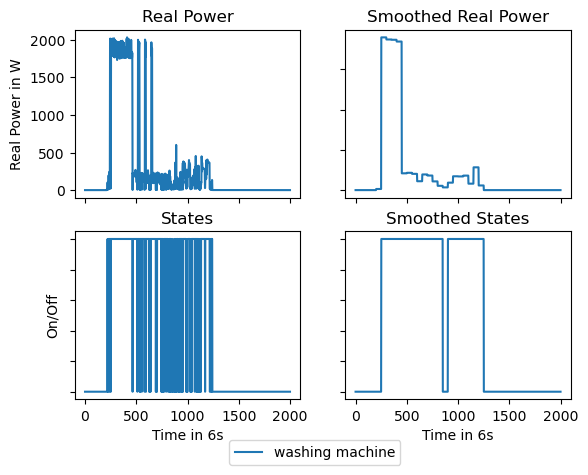
\includegraphics[scale=0.55]{figures/window2.png}
  \label{fig:preprocessing}
\end{figure}

\subsubsection{BLOND}
The preprocessing of the BLOND dataset is similar to the UK-DALE preprocessing. 
BLOND already provides the precomputed one second summery of real power measurements.
Therefore, no resampling and was needed.
Still, two other preprocessing steps had to be applied.

\begin{enumerate}
  \item Find suitable appliances
  \item Find thresholds and window sizes
  \item Create aggregate real power signal
  \item Remove noise with quantile filter
  \item Create ON/OFF states of appliances
  \item Normalizing with std and mean
\end{enumerate}

The measurements of the dataset were recorded over 213 days. 
This resulted in changing appliances.
Some appliances were unplugged or different appliances were plugged in at the same socket during different time periods.
This means that the measurements taken from one socket could contain measurements of different appliances.
Therefore, the first step is to gather appliances with a meaningful load profile that also were measured at the same time.
This way, the appliance usage patterns, like a monitor is used when the corresponding computer is used, are preserved when creating the aggregate signal.

In the next step, the power thresholds and window sizes for each appliance are determined.
The power thresholds and window sizes for the quantile filter are given for the appliances of the UK-DALE dataset, but no information was provided how they were calculated.
Therefore, different combinations of window sizes and thresholds were tested to find a proper visual filtering for each appliance (Assumption 2).
Each combination of window sizes and power thresholds lead to different smoothing of the power signal and also to different ON/OFF states.
One of the applied criteria to find a valid filtering is that laptops or monitors should be in an ON state during most of the working hours.
The figure \ref{fig:window_blond} shows the preprocessing of an MacBook Pro 15'' and the effects of the quantile filter.
The sequence contains data from one week. 

The other steps are similar to the steps presented in section \ref{chapter:preprocessing_ukdale} of the preprocessing on UK-DALE.

\begin{figure}
  \caption{Testing different window sizes and thresholds on BLOND}
  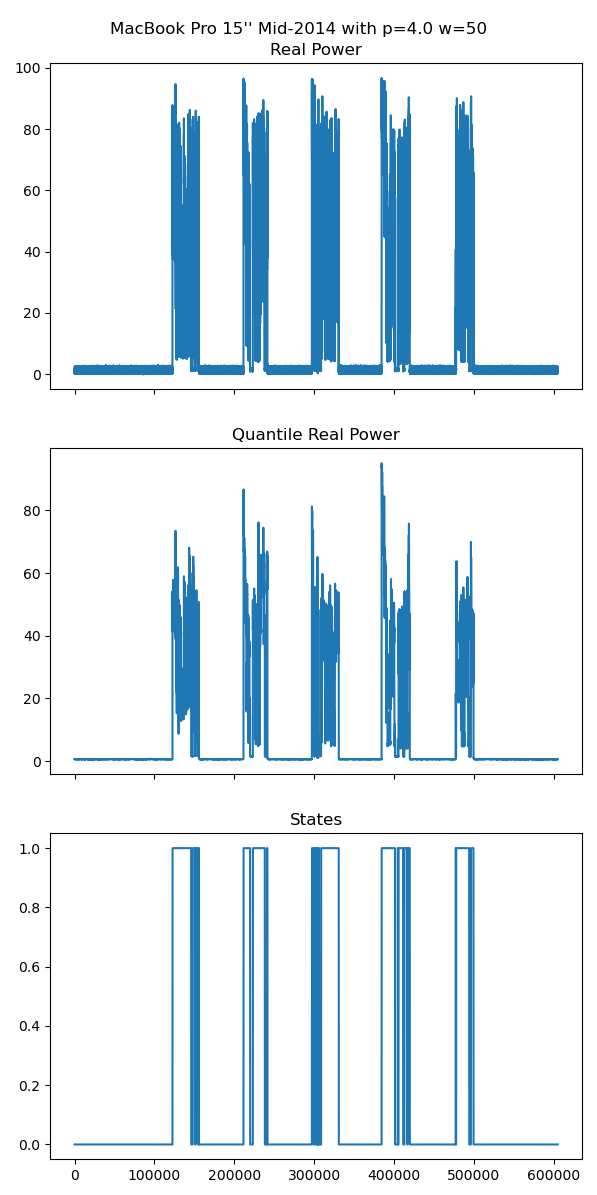
\includegraphics[scale=0.5]{figures/window.png}
  \label{fig:window_blond}
\end{figure}

\subsection{Performance metrics}
In order to compare our reimplementation the same metrics are used as in the original UNet-NILM paper~\cite{unetnilm}.
The metrics used for the regression task are the mean absolute error (MAE), estimated accuracy (EAC) and the normalized disaggregation error (NDE).
The metric used for the multi-label classification task is the example-based $F_1$ score ($F_1$-eb).
The MAE quantifies the absolute error in predicted power at every timestep and is given by:
\begin{equation}
  MAE(y, \hat{y}) = \frac{1}{TM}\sum_{t=1}^{T} \sum_{m=1}^{M} |\hat{y}_m(t) - y_m(t)|
\end{equation}
The EAC measures the total estimated accuracy and is defined as:
\begin{equation}\label{eq:eac}
  \begin{split}
    EAC(y, \hat{y}) &= 1 - \frac{\sum_{t=1}^{T} \sum_{m=1}^{M} |\hat{y}_m(t) - y_m(t)|}{2\sum_{t=1}^{T} \sum_{m=1}^{M} y_m(t)} = \\
                  &= 1 - \frac{TM \times MAE(\hat{y}, y)}{2\sum_{t=1}^{T} \sum_{m=1}^{M} y_m(t)}
  \end{split}
\end{equation}
Lastly the NDE gives the normalized error of the squared differences between the prediction and the ground truth and is defined as:
\begin{equation}\label{eq:nde}
  NDE(y, \hat{y}) = \frac{\sum_{t=1}^{T} \sum_{m=1}^{M} (\hat{y}_m(t) - y_m(t))^2}{2\sum_{t=1}^{T} \sum_{m=1}^{M} y_m(t)^2}
\end{equation}
with $y$ being the ground truth values, $\hat{y}$ the prediction and $T$ and $M$ are the window size and the number of 
appliances respectivly.
For the classification metrics $F_1-eb$ is used, which is an instance based metric that measures the ratio of correctly predicted
labels to the sum of the total true and predicted labels and is defined as:
\begin{equation}
  F_1-eb = \frac{\sum^M_{m=1} 2t_p(m)}{\sum^M_{m=1} s_t + \sum^M_{m=1} \hat{s}_t}
\end{equation}
with $s$ and $\hat{s}$ being the ground truth and predicted states and $M$ being the number of appliances~\cite{unetnilm}.

The value ranges and optimas for each of the metric are: 
$MAE \in [0, +\infty[$ with MAE being optimal when $MAE=0$,
$EAC \in ]-\infty, +\infty[$ with EAC being optimal when $EAC=1$, 
$NDE \in [0, +\infty[$ with NDE being optimal when $NDE=0$
and lastly $F_1 \in [0,1]$ and $F_1$ being optimal when $F_1=1$.

\section{Experiments \& Results}\label{chapter:expiraments}
\subsection{UKDALE}\label{subchapter:ukdale}
In the experiments to test the reimplementation the same set of hyperparameters are used as proposed by Faustine et al.~\cite{unetnilm}.
These hyperparameters include an initial learning rate of $\alpha=0.001$, $\beta=(0.9,0.98)$ and a batch size of $128$. 
As optimizer Adam is used and the learning rate is reduced by a factor of $0.1$ every 5 epochs, if the $F_1$-eb on the 
validation set has not been improved over 5 epochs. This learning rate scheduler is the so called ReduceLROnPlateau scheduler.
Additionally the same quantiles $\tau$ are used as by Faustine et al.~\cite{unetnilm}. These quantiles are $[2.5\%,10\%,50\%,90\%,97.5\%]$. 
Similar to Faustine et al.~\cite{unetnilm} the median of all the quantiles is used as final prediction for computing the metrics.
In this case the median quantile is the $50\%$ quantile.
Regarding the UNet-NILM architecture 7 layers are used, meaning that the network consists of 7 Down-/ and Upsampling blocks.
UNet-NILM and CNN1D were both trained for 100 epochs and trained with a window size of 100 and a slide of 50. 

Convergence on the validation loss started for both models at about epoch 50, see figure~\ref{fig:loss_graphs}.
Figure~\ref{fig:loss_graphs} shows the training and validation loss curves for UNet-NILM, in blue, and 1DCNN, in orange.
For both models the training and validation loss is continuously decreasing, however, for UNet-NILM the validation loss falls at 
epoch 40, resulting in a smaller validation loss in the end for UNet-NILM.

The performance metrics of both models can be seen in table~\ref{tab:unetvscnn1d}. 
Each row in the table shows a appliance with the last row showing the average over all appliances.
Each column in the table shows a metric for the given model in parantheses. 
For certain appliances like the dishwasher and the washing machine UNet-NILM's MAE and NDE is half as great as CNN1D's MAE and NDE.
Regarding the other appliances, the results are mixed. Meaning that CNN1D performs better as UNet-NILM or as well as or underperforms. 
However, in average UNet-NILM outperforms CNN1D in every metric by an order of magnitude.

In comparison to the performance of Faustine et al.'s models, see table~\ref{tab:orginalpaperresults}, it is visible that 
both our CNN1D and our U-Net model perform better than Faustine et al. models, except for the F1-score, where our models underperform with a difference 
of $\sim 0.06$ for CNN1D and $\sim 0.04$ for UNet-NILM. The metrics for the regression task show that our model's results are better than
Faustine et al.'s results with differences in the MAE of $\sim 4$ for CNN1D and UNet-NILM and in the NDE with differences of $\sim 0.13$ for CNN1D and $\sim 0.07$ for UNet-NILM.

In order to see real world application performance, time windows from the test set are disaggregated by our 
UNet-NILM model and our CNN1D model and visualized in order to see a more detailed performance comparsion, see figure~\ref{fig:window1588} to figure~\ref{fig:window1585}. 
For each of these plots the left column contains subplots for the real power and the right column for the states,
while the first row shows the ground truth, the second row the disaggregation prediction of CNN1D and the third row the disaggregation prediction of UNet-NILM.
In each subplot the y-axis shows the power consumption in watts or the state respectively and the x-axis gives the time in the window. 
In figure~\ref{fig:window1588} it is clearly visible, that UNet-NILM does not detect the On/Off event of the kettle. For CNN1D
the estimated power consumption of the kettle is underestimated and an additional On/Off event for the microwave is disaggregated,
which can not be found in the ground truth. 
In figure~\ref{fig:window1586} UNet-NILM disaggregates a non-existing On/Off event for the microwave. Both CNN1D and UNet-NILM correctly disaggregate 
the On/Off event of the kettle, while the predicted real power is increasing step wise, which does not represent the ground truth showing a clear rectangle.
In figure~\ref{fig:window1945} UNet-NILM disaggregates the states correctly with an underestimation of the real power of the washing machine. 
CNN1D's real power estimation for the washing machine is closer to the ground truth than UNet-NILM's, however, CNN1D mispredicts the state of the fridge as off. 
In the last disaggregation plot, seen in figure~\ref{fig:window1585} both CNN1D and UNet-NILM mispredict an On event for the fridge, while 
UNet-NILM also mispredicts an On event for the microwave.

Next different number of layers of the UNet-Block are also tried in order to see if UNet-NILM performs as well as with less parameters.
The results can be seen in figure~\ref{fig:layer_comp} containing 4 subplots each one representing the relation between 
the number of layers used, shown on the x-axis, and the corresponding value for the metric.
For MAE, NDE and EAC a clear peak at 7 down- and upsampling layers is visible. 
This is not the case for the F1-score, where an increase is visible from 4 to 7 and from 7 to 10 the F1-score is decreasing again.
The plots indicate that it is possible that the metrics may plateau from a value of 10 down- and upsampling layers.

\begin{figure}
  \caption{Loss graphs of U-Net and 1DCNN}
  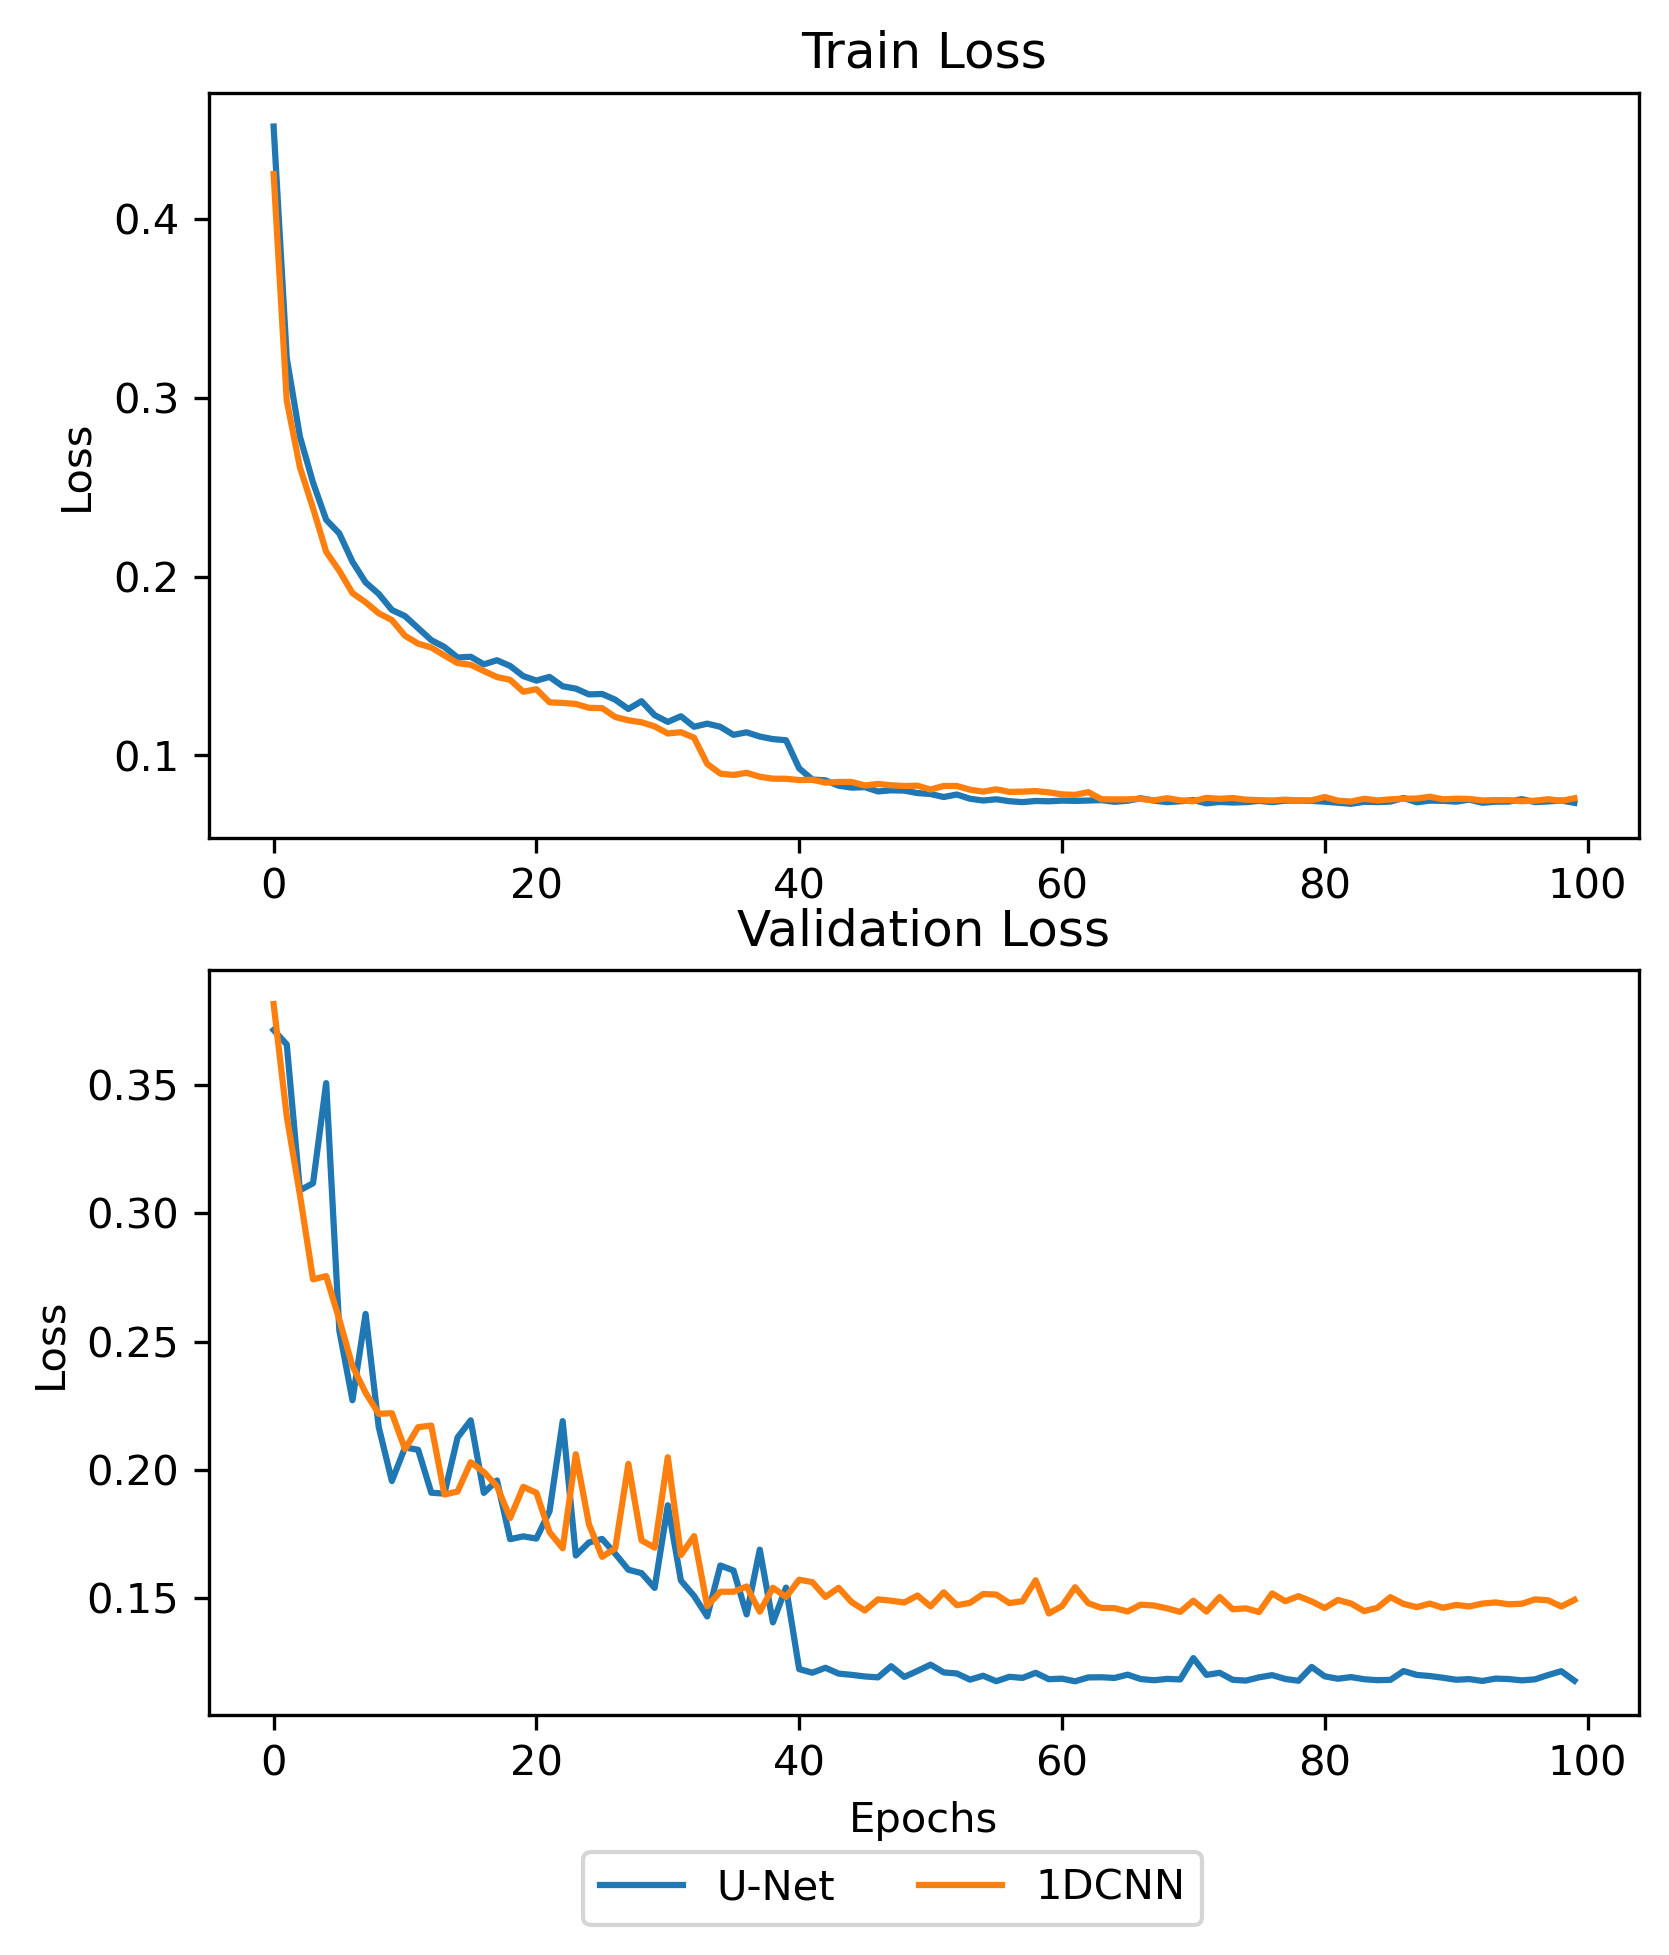
\includegraphics[scale=0.6]{figures/loss_graphs.png}
  \label{fig:loss_graphs}
\end{figure}

\begin{figure}
  \caption{Comparison of different layers}
  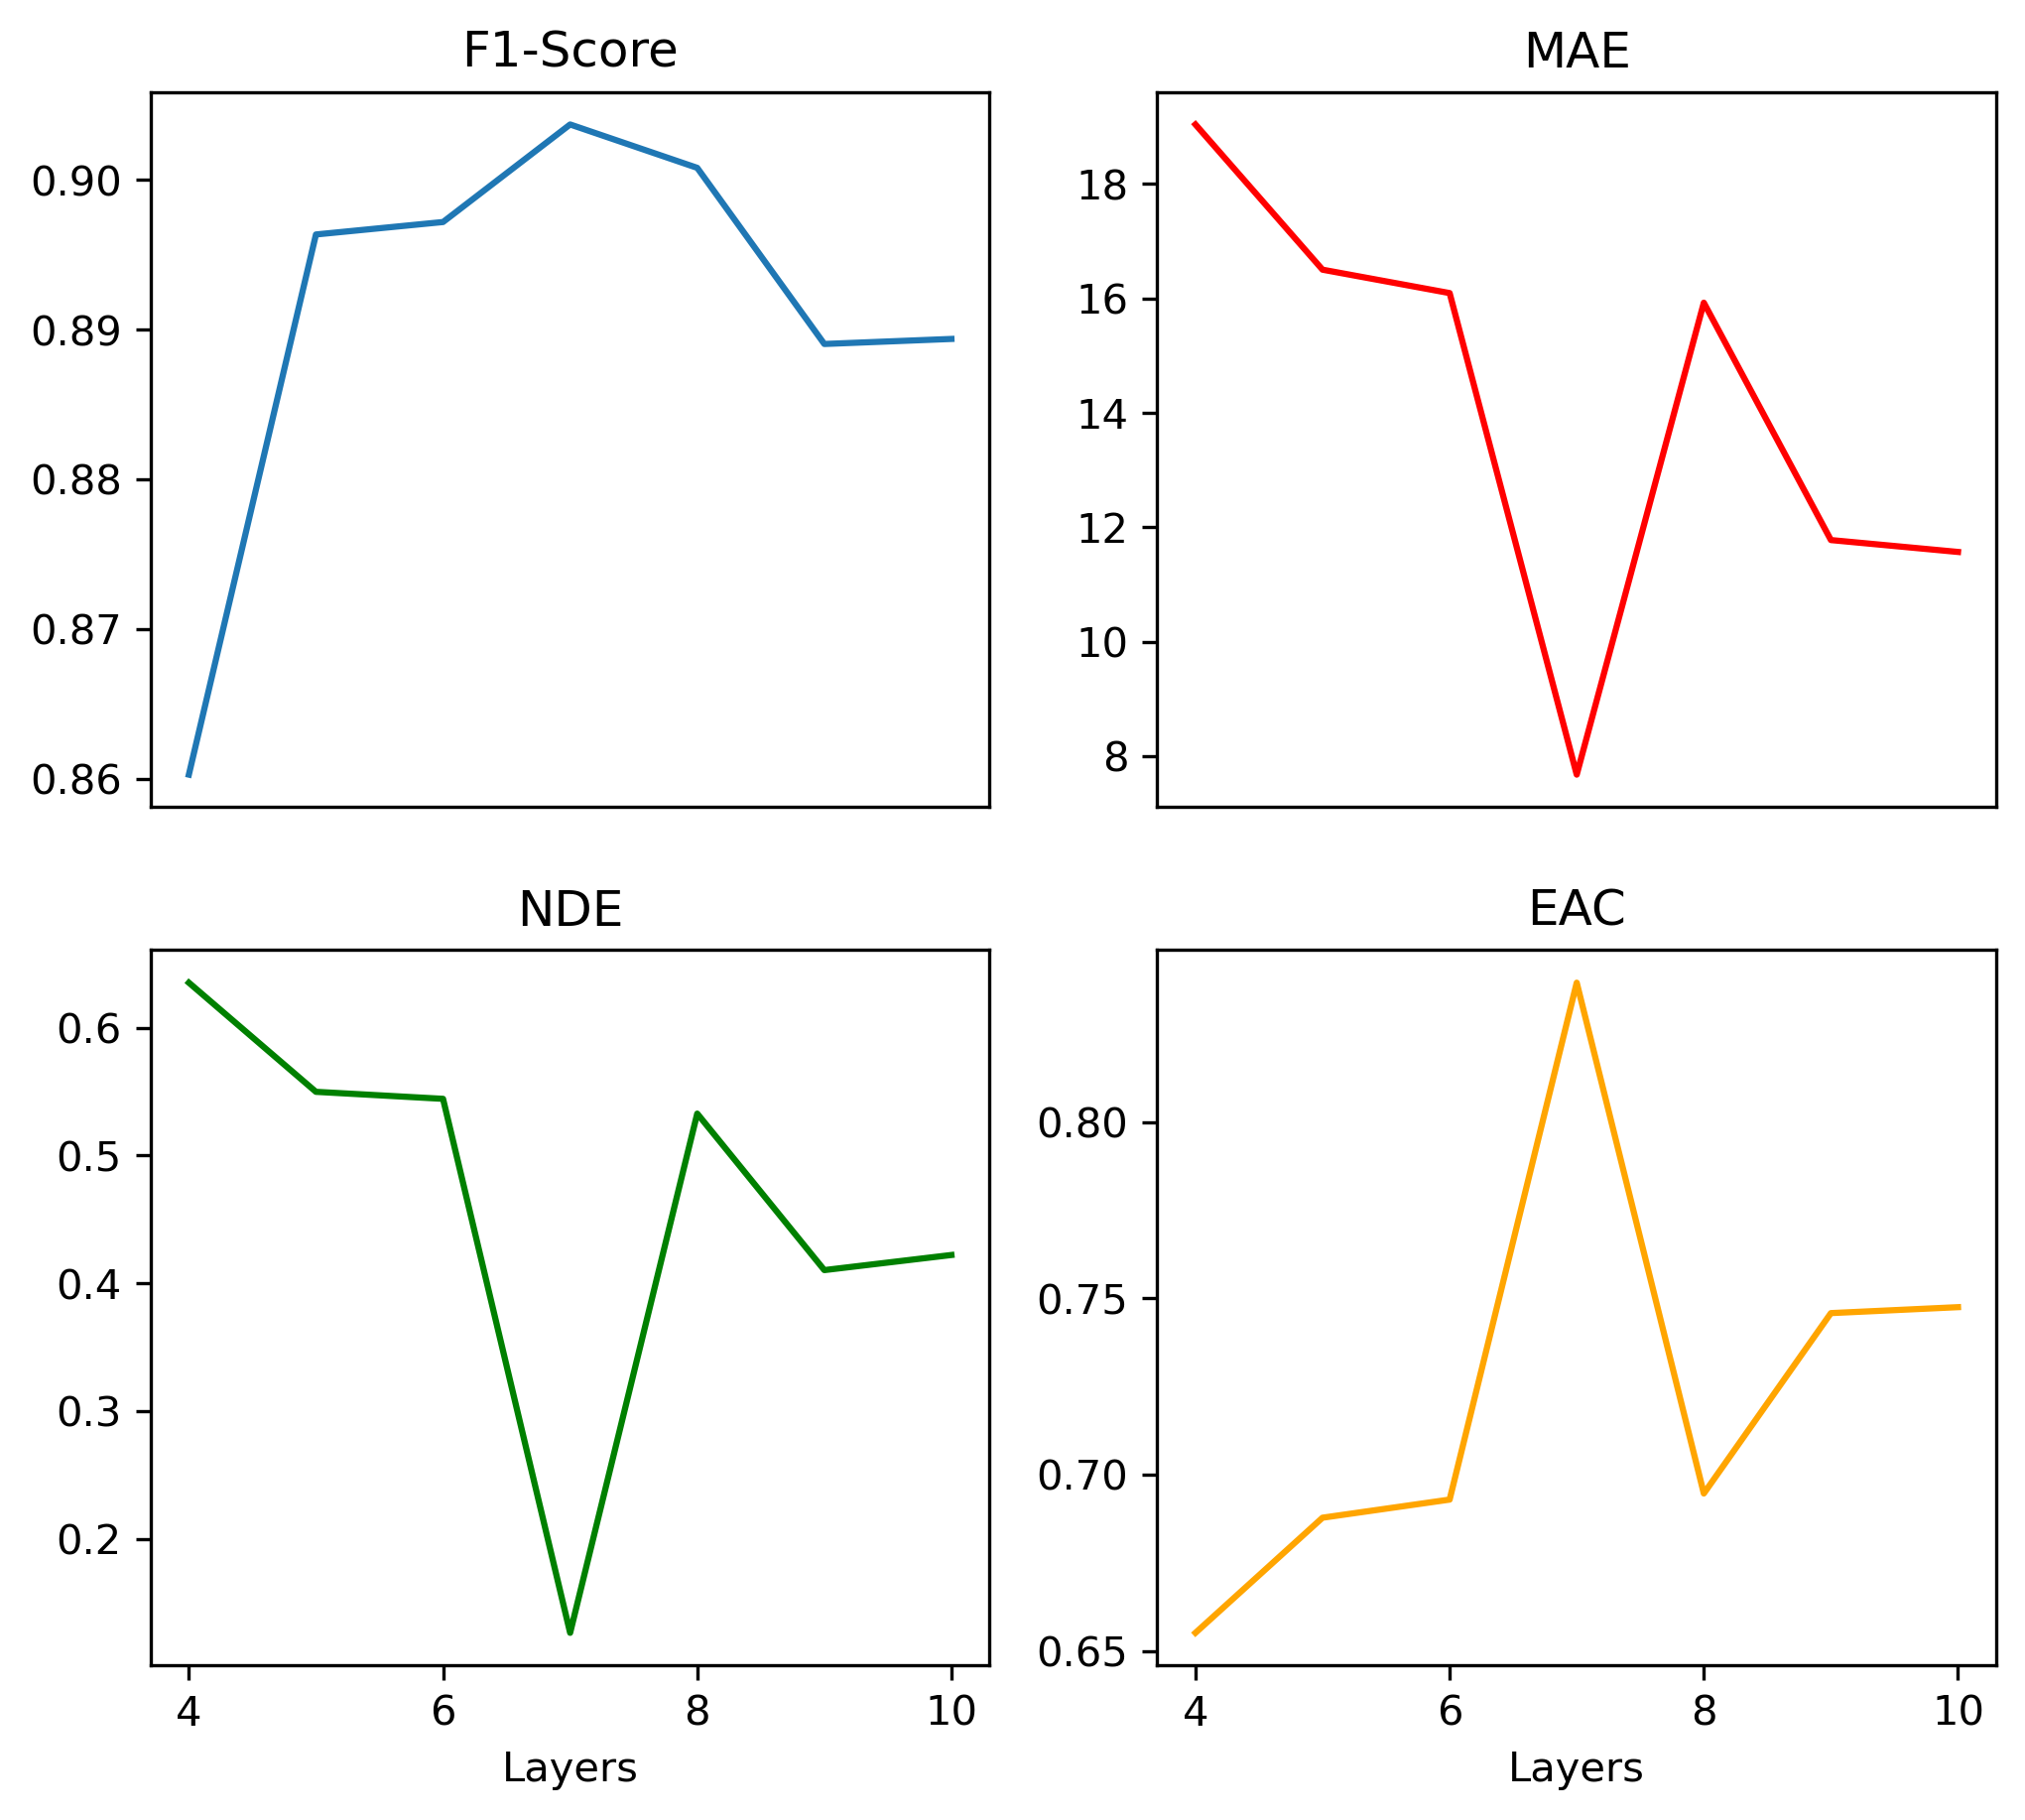
\includegraphics[scale=0.5]{figures/layer_comp.png}
  \label{fig:layer_comp}
\end{figure}

\begin{table*}
  \caption{Results of the reimplementation of the CNN1D approach vs UNet-NILM}
  \label{tab:unetvscnn1d}
  \begin{tabular}{lrrrrrrrr}
    \toprule
    {} &  EAC(CNN1D) &  EAC(UNET) &  F1(CNN1D) &  F1(UNET) &  MAE(CNN1D) &  MAE(UNET) &  NDE(CNN1D) &  NDE(UNET) \\
    \midrule
    washing\_machine &    0.801426 &   0.882215 &   0.930374 &  0.943700 &   13.816046 &   8.195056 &    0.151602 &   0.071262 \\
    dishwasher      &    0.829188 &   0.907923 &   0.822006 &  0.858006 &   14.275379 &   7.695221 &    0.159172 &   0.051244 \\
    kettle          &    0.787865 &   0.773779 &   0.914420 &  0.943128 &    9.735492 &  10.381933 &    0.171687 &   0.156246 \\
    fridge          &    0.909107 &   0.933943 &   0.948937 &  0.957895 &    6.818886 &   4.955684 &    0.096624 &   0.078902 \\
    microwave       &    0.682867 &   0.699524 &   0.778285 &  0.815851 &    7.555889 &   7.159031 &    0.370487 &   0.274331 \\
    AVG             &    0.802090 &   0.839477 &   0.878805 &  0.903716 &   10.440339 &   7.677385 &    0.189915 &   0.126397 \\
    \bottomrule
    \end{tabular}    
\end{table*}

\begin{table*}
  \caption{Original results from Faustine et al.~\cite{unetnilm}}
  \label{tab:orginalpaperresults}
  \begin{tabular}{lrrrrrrrr}
    \toprule
    {} &  EAC(CNN1D) &  EAC(UNET) &  F1(CNN1D) &  F1(UNET) &  MAE(CNN1D) &  MAE(UNET) &  NDE(CNN1D) &  NDE(UNET) \\
    \midrule
    washing\_machine &       0.875 &      0.909 &      0.954 &     0.963 &      15.758 &     11.506 &       0.111 &      0.062 \\
    dishwasher      &       0.875 &      0.914 &      0.913 &     0.909 &       9.884 &      6.764 &       0.126 &      0.080 \\
    kettle          &       0.589 &      0.677 &      0.944 &     0.956 &      20.390 &     16.003 &       0.674 &      0.429 \\
    fridge          &       0.923 &      0.937 &      0.964 &     0.962 &      18.583 &     15.124 &       0.073 &      0.072 \\
    microwave       &       0.630 &      0.753 &      0.907 &     0.916 &       9.690 &      6.475 &       0.656 &      0.334 \\
    AVG             &       0.778 &      0.838 &      0.937 &     0.941 &      14.860 &     11.174 &       0.328 &      0.195 \\
    \bottomrule
    \end{tabular}
\end{table*}

\foreach \i in {1588, 1945, 1586, 1585}
{%
  \begin{figure}
    \caption{UKDALE:time window \i}
    \expandafter\label\expandafter{fig:window\i}
    \noexpand{\includegraphics[scale=0.5]{figures/windows/UKDALE/UNET_CNN1D_\i.png}}
  \end{figure}
}%

\subsection{BLOND}
As a further experiment for UNet-NILM, the model is also trained on the BLOND dataset~\cite{BLOND}, because BLOND is a more difficult dataset, as stated in section~\ref{seciton:datasets:blond}
For the experiments 2,3,4 and 5 appliances are disaggregated and more layers to UNet-NILM are added. 
Since no hyperparameters for training were given this time, grid search over the learning rates $1\times 10^{-3}$, $1\times 10^{-5}$
and $1\times 10^{-7}$ is used, where each model is trained for 20 epochs. 
The optimizer, window size, slide, quantiles and scheduler are the same as for UKDALE, see~\ref{subchapter:ukdale}.
Due to hardware limitations it was not possible to include more hyperparameters to the grid search.

In order to see wether it is possible to fit UNet-NILM to BLOND, the first experiment was to only disaggregate 2 appliances and increase the 
number of appliances by adding new appliances using our best UNet-NILM architecture from UKDALE with 7 down- and 7 upsampling layers. 
The idea behind this method is by incrementing the number of appliances step by step the problem is becoming more complex step by step and therefore one can see
when the model is not complex enough to fit the dataset.
Table~\ref{tab:apps} shows which appliances are used at each step.
For 3 appliances an alternative set of appliances is given, where one appliance is changed in order to see whether the performance drop is 
due to the specific appliance.

The first results showed that the model trained on 5 appliances performs worse than the model trained on 2 appliances, therefore it is worth to see if this 
behaviour is visible during training. Figure~\ref{fig:BLONDloss} shows the train and validation loss curves for the 
model trained on 2 appliances, in blue, and for the model trained on 5 appliances, in orange. 
For both models the training loss curve is continuously decreasing. However, for the model trained on 5 appliances the loss 
is $\sim 0.2$ greater than for the model trained on 2 appliances.
The validation loss curves on the other hand show a more divergent pattern where the validation loss is decreasing for the 2 
appliances model after the 8th epoch and the validation loss curve is not staying stagnant regarding the 5 appliances model.
In the end, the difference between the validation loss curves is $\sim 0.2$, which is similar to the training loss curves.

A performance comparison between the number of appliances can be seen in figure~\ref{fig:apps_comp}.
The figure consists of 4 subplots each showing one metric, which is described by the y-axis, in relation to the number of appliances 
used.
For every metric it holds that adding more appliances to the task, the performance becomes worse.
This is seen by the continuous decreasing F1-score and EAC and increasing NDE.
The MAE is decreasing, which indicates that the predictions become better with more appliances, however, 
regarding the values of the MAE, the difference from best to worst is $\sim 1.5$. This small difference may not be significant,
because the value of the MAE depends heavily on the absolute real power values $y$ and $\hat{y}$. Further investigations 
into this have not been made, since the NDE and the EAC deal with this problem by normalizing the absolute or quadratic difference, 
see equations~\ref{eq:nde} and~\ref{eq:eac}.

A more detailed prediction performance for 2 appliances and 5 appliances can be seen in table~\ref{tab:2apps} and table~\ref{tab:5apps} respectivly.
Looking at table~\ref{tab:2apps} specifically, the model learns the disaggregation of the monitor and laptop extraordinary well,
with the performance for the monitor being outstanding good. This can also be seen for the model trained for 5 appliances in table~\ref{tab:5apps}.
Here the same two appliances are learned almost perfectly with the monitor again being the best predicted appliance.
However, regarding the other 3 appliances, a worse performance is seen with F1-scores of 0.2 for 
the desktop pc and even completly 0 for the projector. 
The projector with a F1-score of 0 is an interesting case, because on the one hand it shows that the model is not capable to predict the correct 
On/Off states for this appliance. On the other hand regarding the power estimation metrics EAC, MAE and NDE show that the model 
is capable of estimating the power consumption of the projector.

More detailed disaggregation results can be seen from figure~\ref{fig:2appswindow1156} to figure~\ref{fig:5appswindow16704}. 
Figure~\ref{fig:2appswindow1156} and figure~\ref{fig:5appswindow1156} show the same window for the 2 appliances model and 5 appliances model respectively.
This specific window is choosen because it contains an On/Off event for the monitor. 
The 2 appliances model disaggregates this window correctly with an accurate real power prediction, while the 5 appliances model sees the On/Off event, however, it missclassifies it 
as projector event. Additionally the 5 appliances model's real power estimations are also far off the ground truth.
Figure~\ref{fig:2appswindow16704} and figure~\ref{fig:5appswindow16704} show the same window for the 2 appliances model and 5 appliances model respectivly and this 
window contains an On/Off event for the laptop.
Here the 2 appliances model and the 5 appliances model completly fail to disaggregate the On/Off event and the real power predictions 
of both models are far off the ground truth.

In order to see whether better performance can be achieved by using our described training method, the model 
complexity is increased by using 10 down-and upsampling blocks in the UNet-Block instead of 7. The 10 layer network is also trained for a 
disaggregation task with 5 appliances. The results can be seen in table~\ref{tab:BLONDlay}. The difference in performance between 
the 10 layer and 7 layer models is marginal for every metric for each appliance.

\begin{figure}
  \caption{Train and validation loss graphs of UNet-NILM trained on 5 appliances}
  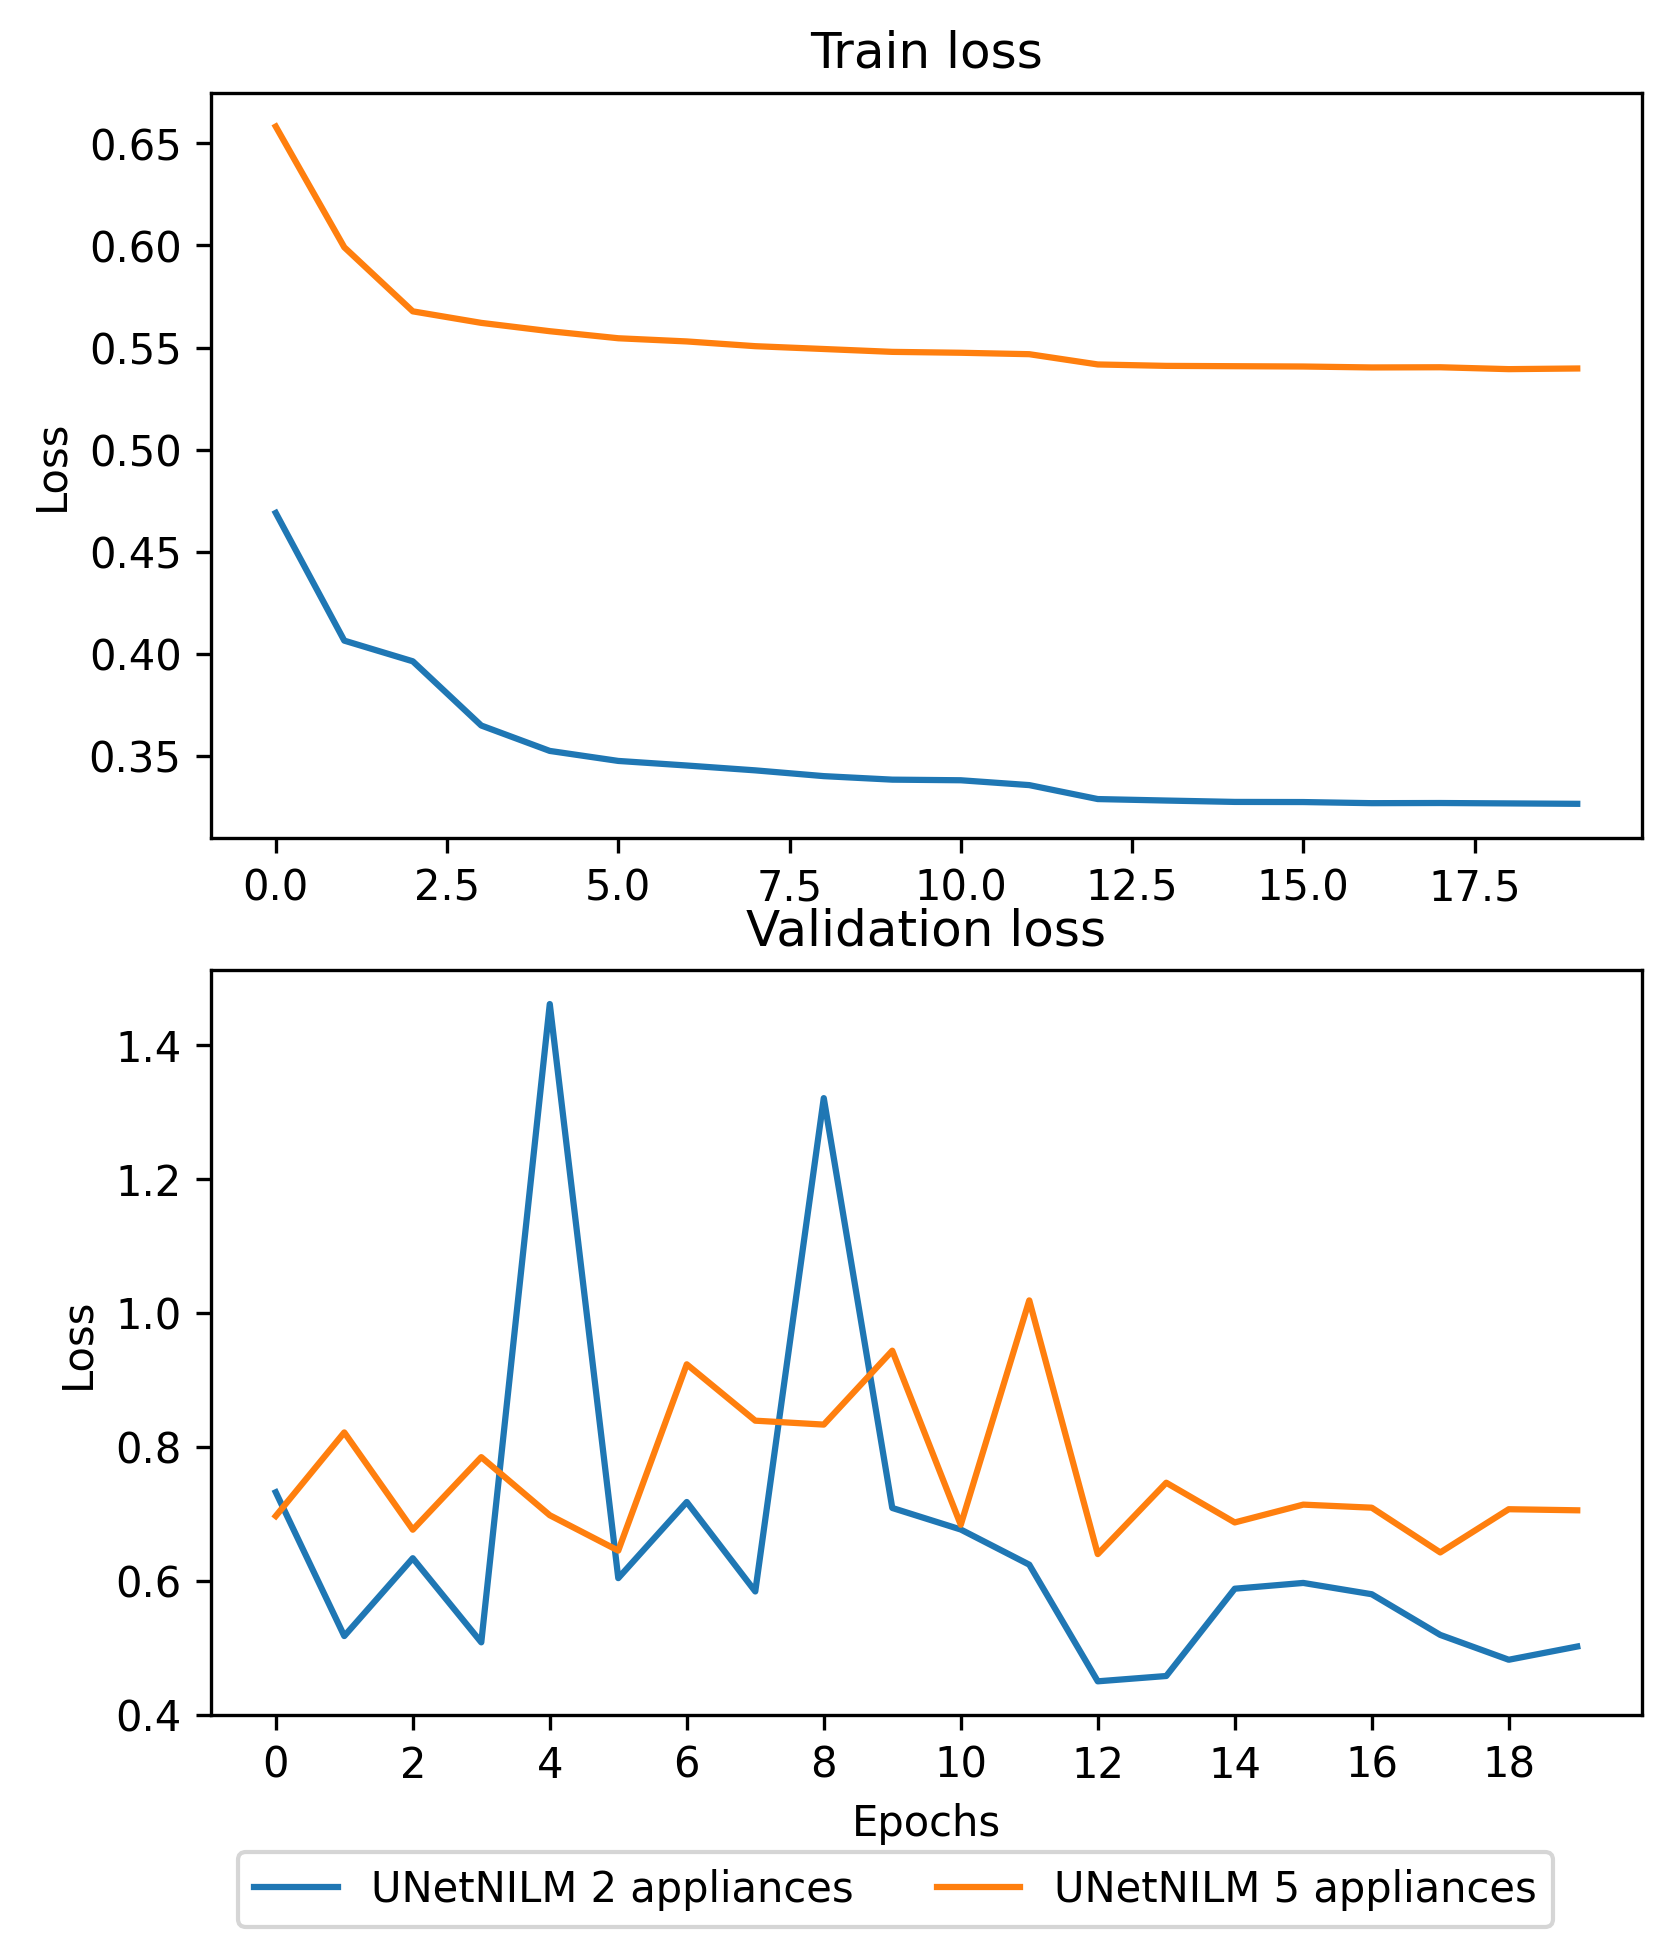
\includegraphics[scale=0.6]{figures/BLOND_loss_graphs.png}
  \label{fig:BLONDloss}
\end{figure}

\begin{table*}
  \caption{Appliance table for the different number of appliances}
  \label{tab:apps}
  \begin{tabular}{ll}
    \hline\hline
    \toprule
    Number of appliances & Appliances \\
    \hline
    \midrule
    2               &                                               Dell U2711, MacBook Pro 15 Mid-2014 \\
    3                &                               Dell U2711, Lenovo X230 i7, MacBook Pro 15 Mid-2014 \\
    3 (alternative)  &                                  Dell U2711, Lenovo T420, MacBook Pro 15 Mid-2014 \\
    4                &                  Dell U2711, Epson EB-65950, Lenovo T420, MacBook Pro 15 Mid-2014 \\
    5               &  Dell U2711, Epson EB-65950, Lenovo T420, Lenovo X230 i7, MacBook Pro 15 Mid-2014 \\
    \bottomrule
    \end{tabular}
\end{table*}

\begin{table*}
  \caption{Per appliance performance results for 2 appliances}
  \label{tab:2apps}
  \begin{tabular}{lrrrr}
    \hline\hline
    \toprule
    {} &       EAC &        F1 &       MAE &       NDE \\
    \hline
    \midrule
    Dell U2711              &  0.989415 &  1.000000 &  1.463026 &  0.000482 \\
    MacBook Pro 15 Mid-2014 &  0.613822 &  0.735266 &  5.641059 &  0.541606 \\ \hline
    AVG                     &  0.801618 &  0.867633 &  3.552042 &  0.271044 \\
    \bottomrule
    \end{tabular}
\end{table*}

\begin{table*}
  \caption{Per appliance performance results for 5 appliances}
  \label{tab:5apps}
  \begin{tabular}{lrrrr}
    \hline\hline
    \toprule
    {} &       EAC &        F1 &       MAE &       NDE \\
    \hline
    \midrule
    Lenovo T420             &  0.609212 &  0.015323 &  3.854207 &  0.922815 \\
    Dell U2711              &  0.994585 &  0.999993 &  0.748348 &  0.000155 \\
    MacBook Pro 15 Mid-2014 &  0.614051 &  0.724138 &  5.637714 &  0.534407 \\
    Epson EB-65950          &  0.913129 &  0.000000 &  0.996063 &  0.889711 \\
    Lenovo X230 i7          &  0.628240 &  0.206640 &  1.159842 &  0.846144 \\ \hline
    AVG                     &  0.751844 &  0.389219 &  2.479235 &  0.638646 \\
    \bottomrule
    \end{tabular}    
\end{table*}

\begin{figure}
  \caption{Comparison of different appliances}
  \label{fig:apps_comp}
  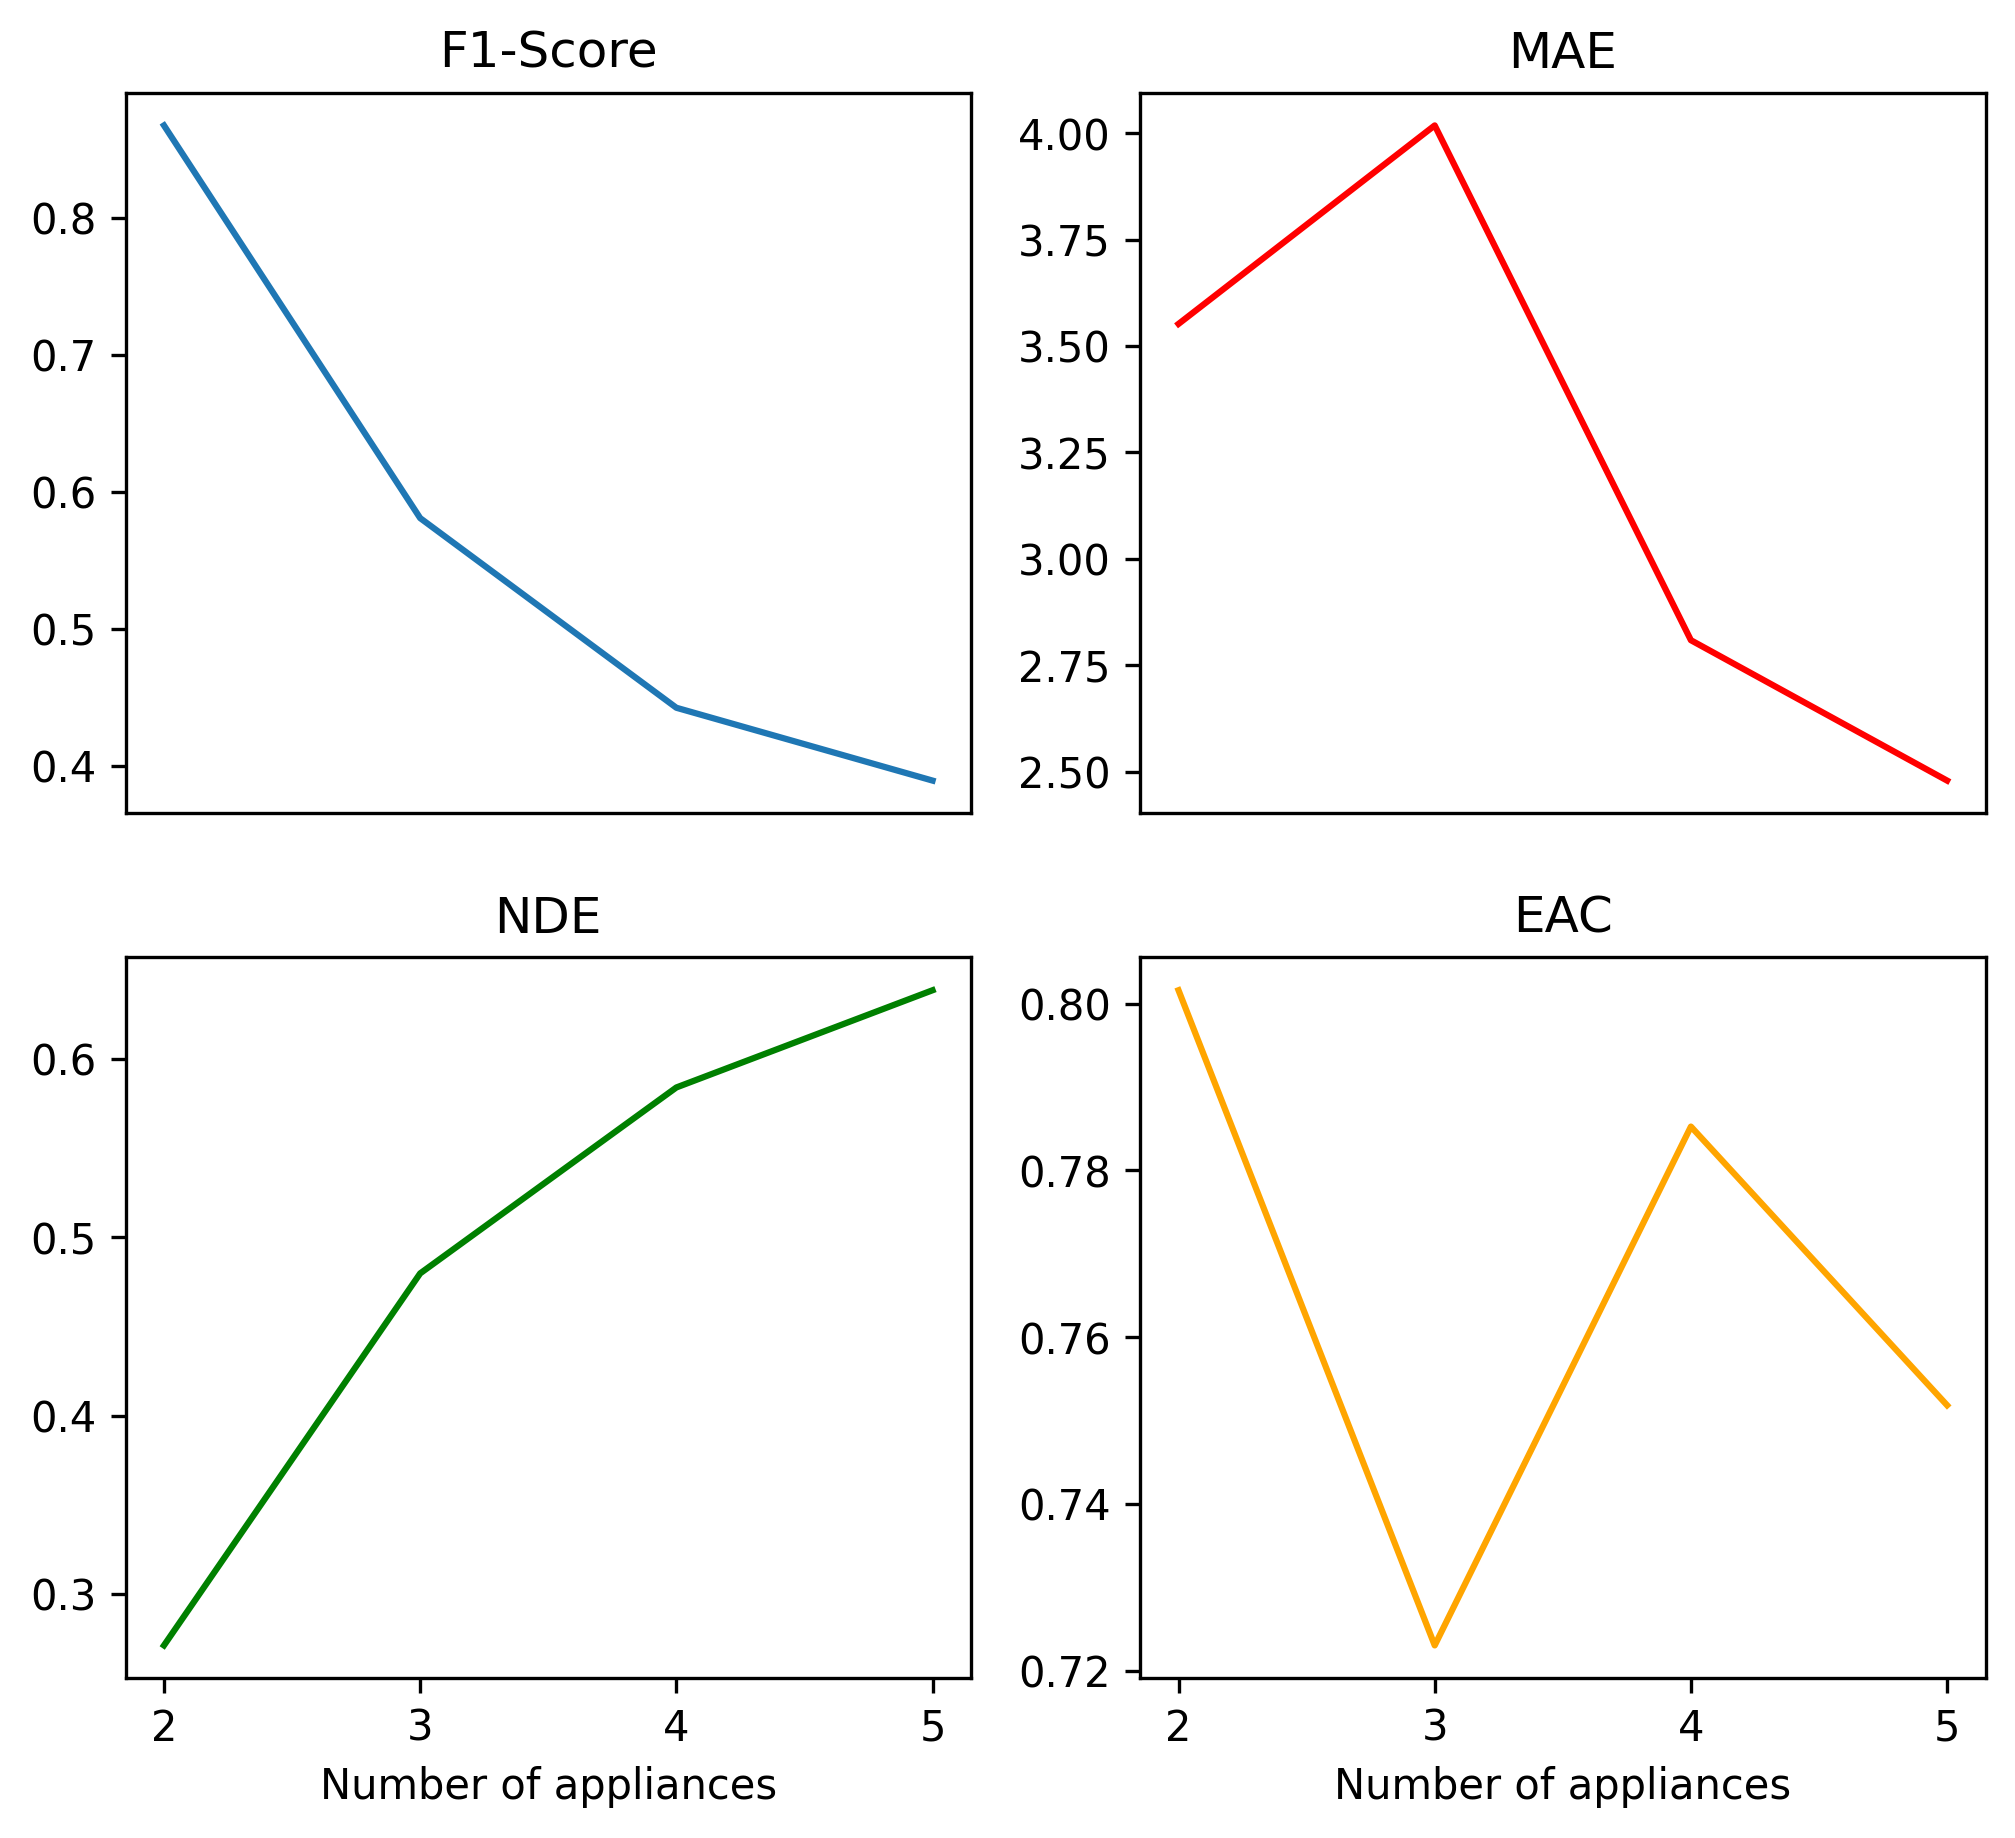
\includegraphics[scale=0.5]{figures/app_comp.png}
\end{figure}

\foreach \i in {1156, 16704}
{%
  \begin{figure}
    \caption{BLOND:time window \i \ for 2 appliances}
    \expandafter\label\expandafter{fig:2appswindow\i}
    \noexpand{\includegraphics[scale=0.5]{figures/windows/BLOND/2apps/UNET_\i.png}}
  \end{figure}

  \begin{figure}
    \caption{BLOND:time window \i \ for 5 appliances}
    \expandafter\label\expandafter{fig:5appswindow\i}
    \noexpand{\includegraphics[scale=0.5]{figures/windows/BLOND/5apps/UNET_\i.png}}
  \end{figure}
}%

\begin{table*}
  \caption{Comparison between UNet-NILM trained on BLOND with 7 and 10 layers}
  \label{tab:BLONDlay}
  \begin{tabular}{lrrrrrrrr}
    \hline\hline
    \toprule
    {} &  EAC(10 layer) &  EAC(7 layer) &  F1(10 layer) &  F1(7 layer) &  MAE(10 layer) &  MAE(7 layer) &  NDE(10 layer) &  NDE(7 layer) \\
    \hline
    \midrule
    Lenovo T420             &       0.601529 &      0.609212 &      0.015691 &     0.015323 &       3.929980 &      3.854207 &       0.889847 &      0.922815 \\
    Dell U2711              &       0.994034 &      0.994585 &      0.999948 &     0.999993 &       0.824613 &      0.748348 &       0.000211 &      0.000155 \\
    MacBook Pro  &       0.610804 &      0.614051 &      0.753815 &     0.724138 &       5.685140 &      5.637714 &       0.527110 &      0.534407 \\
    Epson EB-65950          &       0.913981 &      0.913129 &      0.000000 &     0.000000 &       0.986295 &      0.996063 &       0.889257 &      0.889711 \\
    Lenovo X230 i7          &       0.616802 &      0.628240 &      0.073737 &     0.206640 &       1.195529 &      1.159842 &       0.847421 &      0.846144 \\
    \hline
    AVG                     &       0.747430 &      0.751844 &      0.368638 &     0.389219 &       2.524311 &      2.479235 &       0.630769 &      0.638646 \\
    \bottomrule
    \end{tabular}    
\end{table*}

\section{Discussion}\label{chapter:discussion}
Our first results on the UKDALE dataset show that the results from Faustine et al.~\cite{unetnilm} are reproduceable and our reimplementation is correctly
implemented. Our results outperform Faustine et al.'s results, which may be due to the fact that our models are trained for 100 epochs instead of 50.
Our additional direct disaggregation visualizations show that UNet-NILM and CNN1D do not perfectly predict On/Off events neither estimate the real power correctly. 
The mistakes can be seen on different windows where UNet-NILM has a better disaggregation while CNN1D does not and vice versa
This means that the choosen windows are not too complicated and the mistakes are not data related.
However, when evaluating using only performance metrics UNet-NILM outperforms CNN1D, which is similar to Faustine et al.'s results.

The additional experiment on UKDALE using different number of down-and upsampling blocks in the UNet-Block show that there
is an optimum and an increase in model complexity decreases the model performance and less blocks show a significal 
performance drop. The small difference between 9 and 10 layers may indicate a plateau when further increasing the model complexity.

Our second results on the BLOND dataset show that UNet-NILM is not capable of learning the disaggregation task on a more complicated 
dataset using a similar training method to UKDALE. 
For a small set of appliances it is possible to achieve respectable results for the same UNet-NILM architecture as for UKDALE.
When adding more appliances to the task a clear drop in prediction quality can be seen. A deeper look into these results show that the
performance heavily depends on the appliances, since there are 2 appliances which are predicted correctly, while the model fails to learn to 
disaggregate the other 3 appliances.
Since the task of the model is to learn the behaviour of the appliances, these results indicate that there is a need for a different or more 
complex architecture, which is capable of learning more complex appliances or the data has to be preprocessed differently, since the BLOND data 
used has a sampling rate of 1 Hz, which is a 6 times higher resolution than UKDALE. 
The shown disaggregation windows on the BLOND dataset, support both the argument for a different or more complex architecture and a different 
data preprocessing. The train and validation loss curves also indicate that the problem occurs during the training and not during inference.

The results with a small increase of complexity in the model architecture show that the small increase had no effect on the prediction 
performance. This result supports the argument that the data needs to be preprocessed differently.

Additionally, the results on the BLOND dataset may also come due to the hardware and time limitations. Due to these limitations it was only possible 
to train for 20 epochs, searched for a limited hyperparameter space and tried a limited amount of layers. 

\section{Conclusion}\label{chapter:conclusion}
In conclusion, this paper shows that the results of Faustine et al. are reproduceable and an optimal architecture 
for UNet-NILM in order to fit the UKDALE dataset has been found. This paper also shows that fitting UNet-NILM on BLOND requires a new and full parameter 
search, where the model complexity has to be included in the search space. 

This paper also shows the UNet-NILM approach in more detail including the preprocessing steps for the training data for UKDALE and for BLOND. 
Additionally, a more detailed insight into the prediction performance of UNet-NILM and CNN1D is provided. 

For future work we propose to increase the space of hyperparameters by trying different window sizes,
slides, learning rates, appliances and model complexities and to train UNet-NILM on other datasets 
like BLUED~\cite{BLUED}, REDD~\cite{Kolter2011REDDA}, PLAID~\cite{Gao2014PLAIDAP} or WHITED-A~\cite{Kahl2016WHITEDAWH}.
Additionally, we propose to change the preprocessing of BLOND due to the higher resolution. The changes in preprocessing may vary from 
using a different window size for the appliances for quantile computing to using higher sampling rates in the kHz magnitude, which BLOND provides.

\bibliographystyle{acm}
\bibliography{bib.bib}
\end{document}